\documentclass[12pt,a4paper]{article}
\usepackage[utf8]{inputenc}
\usepackage{amsmath}
\usepackage{amsfonts}
\usepackage{amssymb}
\usepackage{makeidx}
\usepackage{graphicx}
\usepackage{lmodern}
\usepackage{url}
\usepackage{bm}
\usepackage{color}
\usepackage{booktabs}
\usepackage{float}
\usepackage[left=2cm,right=2cm,top=2cm,bottom=2cm]{geometry}
\author{Mudathir Mahgoub}
\title{Project report}
\begin{document}

\maketitle

\section{Description of PDL solver}
This PDL solver checks the satisfiability of formulas in propositional dynamic logic (PDL).
The input is a kripke frame, which is optional, followed by a formula in PDL. The output is the satisfiability result of this formula which is either \textit{unsat}, \textit{sat} or \textit{unknown}. If the result is \textit{sat}, the solver outputs a kripke frame that satisfies the formula. Furthermore, it specifies the set of states where the formula is satisfied. If this set is equal to $K$, the set of all states in the kripke frame, then the formula is valid in this kripke frame. Otherwise, this set satisfies the formula and its complement, with respect to $K$, falsifies the formula. 

To check the validity of a formula in all kripke frames, its negation should be used as an input and if the result is \textit{unsat}, then it is valid. If the result is \textit{sat}, then the returned kripke frame is a counter example that falsifies the original formula.

\section{PDL Complexity}

The satisfiability problem for PDL formulas is decidable, and it is \textit{EXPTIME-complete} (theorm 8.5 in \cite{dynamic}). Therefore the solver may fail to determine the satisfiability within the time limit (by default it is 30 seconds), and hence it returns \textit{unknown} result. 

% THEOREM 6.5 ( SMALL MODEL THEOREM): Let $\varphi$ be a satisfiable formula of
% PDL. Then $\varphi$ is satisfied in a Kripke frame with no more than $2^{\vert \varphi \vert}$ % states.

On the other hand the satisfiability of a PDL formula in a given Kripke frame can be determined in polynomial time (exercise 6.4 in \cite{dynamic}). So one expects this to be easy for CVC4 when the model (Kripke frame) is given and ``check-sat" is executed. Unfortunately, CVC4 doesn't terminate if the formula is \textit{unsat} and uses transitive closure operation. After asking an expert (Andrew Reynolds), apparently CVC4 keeps  ``adding a repeating pattern of lemmas related to transitive closure" which needs to be reviewed. Fortunately I found a work around by just removing the constraint related to the PDL formula and asserting only the frame constraints. After CVC4 finds the model, the PDL formula is evaluated. If the result is true, then it is \textit{sat}, otherwise it is \textit{unsat}.


\subsection{Exercise 6.4}

 The following is my reasoning for this exercise where $K$ is the set of all states in the frame:
\begin{itemize}
\item Formulas $\textbf{0}$, $\textbf{1}$, and atomic propositions are subsets of $K$, therefore they can be computed in $O(\vert K \vert)$.
\item Programs $\textbf{skip}?$, $\textbf{fail}?$, and atomic programs are subsets of $K \times K$, therefore they can be computed in $O(\vert K \vert^2)$.

\item Boolean operators $\neg, \wedge, \vee, \rightarrow, \leftrightarrow$ involve set operations $-, \cap, \cup: \mathbb{P}(K) \times \mathbb{P}(K) \rightarrow \mathbb{P}(K)$ where $\mathbb{P}$ denotes the power set. These set operations be computed in $O(\vert K \vert^2)$ or $O(\vert K \vert)$ if hash tables are used.

\item Program operators $;, \cup, *$ and modal operators $[], \langle \rangle$ involve set operations and relation operations $\circ, *: \mathbb{P}(K \times K) \times \mathbb{P}(K \times K) \rightarrow \mathbb{P}(K \times K)$. Both $\circ$ and $*$ can be computed using graph data structures and DFS algorithm. 
For $\circ$ operation, the DFS algorithm stops at depth 2, and for $*$ it continues until the end. 
If the graph is dense, both operations $\circ, *$ require at most $O(\vert K \vert^3)$ to be computed for all states (all graph vertices). 

\item If the number of operators in a given formula $\varphi$ is $n$, then the formula semantics $m(\varphi)$ can be evaluated in $O(n \vert K \vert ^3)$. Finally it takes constant time to evaluate $m(\varphi) \neq \varphi$ to  determine the satisfiability answer. 
\end{itemize}

From the above discussion, the worst case scenario takes $O(n \vert K \vert ^3)$ time which is polynomial. 

\section{Installation}

The following commands download the source code from github and compile it to generate the solver file ``pdl.jar". 

\begin{verbatim}
git clone https://github.com/mudathirmahgoub/pdl
cd pdl
chmod 777 gradlew
./gradlew build
cd bin
chmod 777 cvc4_linux
java -jar pdl.jar -i test.pdl 
java -jar plantuml.jar test.dot
\end{verbatim}

The last command ``java -jar plantuml.jar test.dot" requires graphvis to be in the path. Installation instructions for graphvis are available in \url{https://graphviz.gitlab.io/download/}. 

\section{Software components}
\begin{figure}[H]
\center
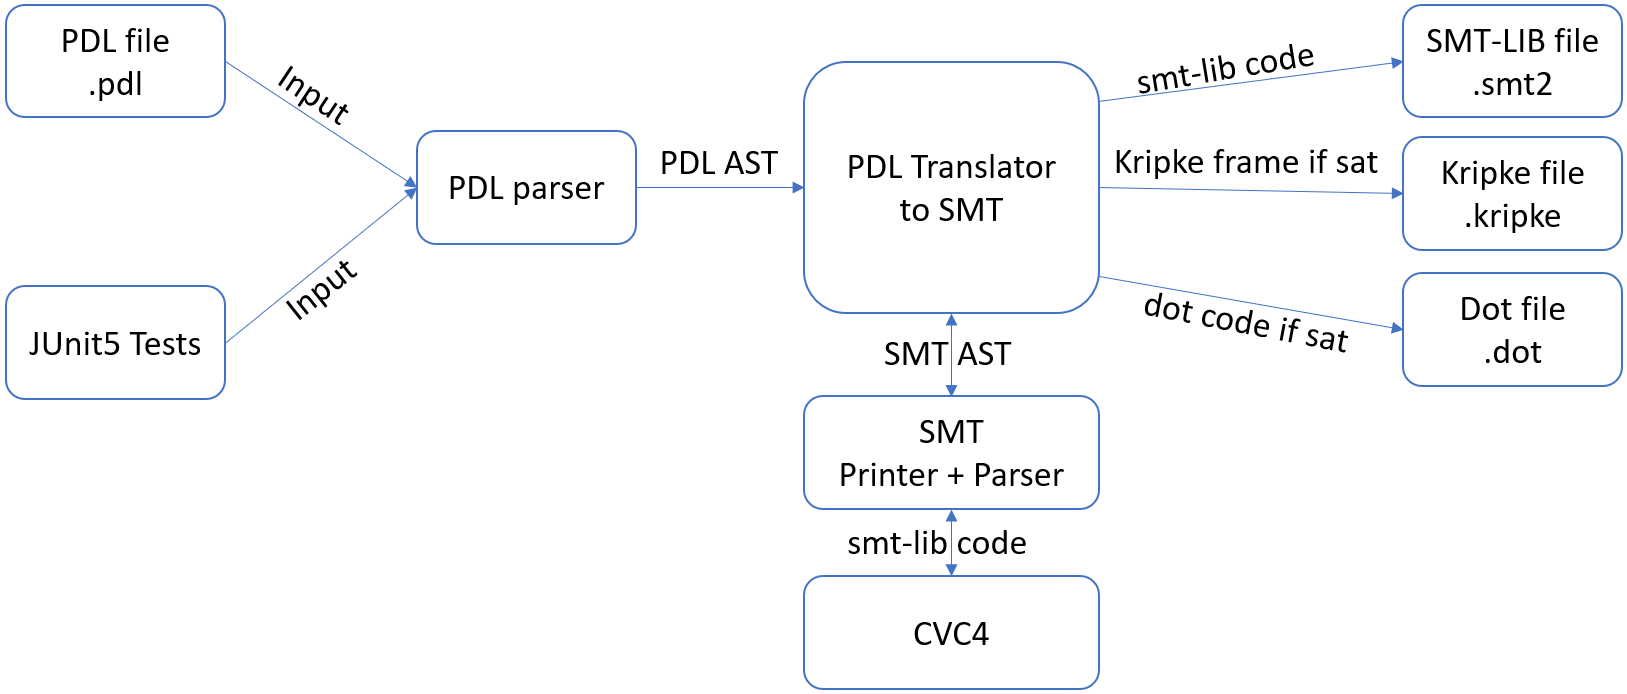
\includegraphics[scale=0.35]{solver.png}
\caption{Software components}
\end{figure}

As shown in the figure above, the input string is parsed into PDL abstract syntax tree (AST) which is read by the translator. Then it gets translated into SMT AST which is sent to CVC4 as SMT-LIB code. CVC4 checks the satisfiability and returns either \textit{sat}, \textit{unsat} or \textit{unknown}. When \textit{sat} result is returned, CVC4 is asked to return the SMT model and the values of additional SMT expressions. The returned SMT model and values are parsed into SMT ASTs which are converted into a kripke frame and a set of states satisfied by the PDL formula. Finally kripke, and dot files are generated. 

The project is written in Java 8 and available in github\footnote{\url{https://github.com/mudathirmahgoub/pdl}}. To build the project, Gradle is used to download and compile the project and generate the jar files. Graphviz software is needed to visualize the generated dot file\footnote{\url{https://www.graphviz.org}}. 

\section{PDL formula translation}

What does it mean to have a satisfiable formula in PDL ?

A PDL formula $\varphi$ is satisfiable if there exists a kripke frame $\mathfrak{K}=(K, m_{\mathfrak{K}})$ and a state  $u$ such that $u \in m_{\mathfrak{K}}(\varphi) $, and we write $\mathfrak{K}, u \models \varphi$. In simple words, a formula is satisfiable if its meaning is nonempty in some kripke frame (i.e. $m_{\mathfrak{K}}(\varphi) \neq \phi$). 

Since the PDL semantics uses set and relation operations, they are translated directly into their corresponding operations in the relation theory in CVC4. The only exception is the reflexive transitive closure $*$ which is not supported directly in CVC4, but supported through the built-in transitive closure. Table \ref{tab:translation} summarizes this translation. Other PDL operators are defined using the basic operators in table \ref{tab:translation}. The book \cite{dynamic} introduces the converse operator $^{\_}$ in page 177 for \textit{backtracking} programs which was not covered in class. Its semantics is the transpose relation which is defined as:
\begin{align*}
m_{\mathfrak{K}}(a^{\_}) = m_{\mathfrak{K}}(a)^{\_} = \lbrace (v, u) \; \vert \; (u, v) \in m_{\mathfrak{K}}(a) \rbrace
\end{align*}


\begin{table}[H]
\begin{center}
\begin{tabular}{ll} 
\toprule
PDL & CVC4 \\    
\midrule    
$K=\lbrace u_0, u_1, \cdots u_n \rbrace$ &  
$\begin{matrix}
\text{\textbf{Atom} : \text{Uninterpreted sort}} \\
u_0, u_1, \cdots, u_n: \textbf{Atom} \\
\textit{atomUniverse}: \text{Set(Tuple (\textbf{Atom}))} = \lbrace \langle u_0 \rangle, \langle u_1 \rangle, \cdots , \langle u_n \rangle \rbrace \\
\textit{atomIdentity}:  = \lbrace \langle u_0, u_0 \rangle, \langle u_1, u_1 \rangle, \cdots , \langle u_n, u_n \rangle \rbrace \\
\end{matrix}$ \\ \midrule   
\textbf{0} & \textit{emptyset} : (Set (Tuple \textbf{Atom})) \\
\textbf{1} & \textit{atomUniverse} \\
Atomic propositions $p, q, r, \cdots$ & $p, q, r, \cdots : \text{Set(Tuple (\textbf{Atom}))}$ \\
Atomic programs $a, b, c, \cdots$ & $a, b, c \cdots : \text{Set(Tuple (\textbf{Atom}$,$\textbf{Atom}))}$ \\
$p \vee q$ & $p \cup q$ \\
$p \wedge q$ & $p \cap q$ \\
$\neg p$ & $\textit{atomUniverse} - p$ \\
$p \rightarrow q$ & $(\textit{atomUniverse}- p)\cup q$ \\
$a;b$ & $a \circ b$ where $\circ$ is the join operator\\
$a \cup b$ (choice) & $a \cup b$ (union)\\
$a^*$ (iteration) & $\textit{atomIdentity} \cup a^+$, (transitive closure)\\
$p?$ (test) & $(p \times p) \cap \textit{atomIdentity}$\\
\color{red}
$a^{\_}$ (converse) & \color{red} $a^t (transpose)$\\

\bottomrule
\end{tabular}
\end{center}
\caption{PDL translation to CVC4.} \label{tab:translation}
\end{table}

\subsection{The semantics of the equivalence operator $\leftrightarrow$}

The textbook \cite{dynamic} did not mention explicitly the semantics of the operator $\leftrightarrow$. However in theorem 5.8 (and other theorems), the book proves the validity of the formula
\begin{align*}
\langle \alpha \cup \beta \rangle \varphi \leftrightarrow \langle \alpha \rangle \varphi \vee \langle \beta \rangle \varphi
\end{align*}
by proving this set equality 
\begin{align*}
m_\mathfrak{K}( \langle \alpha \cup \beta \rangle \varphi ) = m_\mathfrak{K}(\langle \alpha \rangle\varphi  \vee  \langle \beta \rangle \varphi)
\end{align*}

This set equality $=_{\mathbb{P}(K)} : \mathbb{P}(K) \times \mathbb{P}(K) \rightarrow \lbrace \textit{true, false} \rbrace$ ($\mathbb{P}(K)$ is the power set of $K$) is an operation that returns a boolean. This is different than the semantics of operators $\rightarrow, \wedge, \vee: \mathbb{P}(K) \times \mathbb{P}(K) \rightarrow \mathbb{P}(K)$ which returns a subset of $K$. It is possible to use the set equality in $CVC4$ with an $ite$ (\textit{if-then-else}) expression to return a subset of $K$ as follows: 
\begin{align*}
m_\mathfrak{K} (p \leftrightarrow q) = ite(m_\mathfrak{K} (p) =  m_\mathfrak{K}(q), K,  K - \left( (m_\mathfrak{K}(p) - m_\mathfrak{K}(q))  \cup 
   (m_\mathfrak{K}(q) - m_\mathfrak{K}(p)) \right)) 
\end{align*}

In my translation, however,  I used the following semantics:
\begin{align*}
m_\mathfrak{K} (p \leftrightarrow q) = m_\mathfrak{K} ((p \rightarrow q) \wedge (q \rightarrow p))
\end{align*}
The following two lemmas connect between these three approaches in PDL formulas. 

\subsection*{Lemma 1}

\begin{align*}
m_\mathfrak{K} ((p \rightarrow q) \wedge (q \rightarrow p)) = ite(m_\mathfrak{K} (p) =  m_\mathfrak{K}(q), K,  K - \left( (m_\mathfrak{K}(p) - m_\mathfrak{K}(q))  \cup 
   (m_\mathfrak{K}(q) - m_\mathfrak{K}(p)) \right)) 
\end{align*}
\subsubsection*{\textit{Proof}}
\begin{enumerate}
\item Case $m_\mathfrak{K} (p) =  m_\mathfrak{K}(q)$:
\begin{align*}
m_\mathfrak{K} ((p \rightarrow q) \wedge (q \rightarrow p)) &= 
((K - m_\mathfrak{K}(p)) \cup m_\mathfrak{K} (q)) \cap 
((K - m_\mathfrak{K}(p)) \cup m_\mathfrak{K} (q)) \\
&= K \cap K  \\
&=K  = ite(m_\mathfrak{K} (p) =  m_\mathfrak{K}(q), K,  K - \left( (m_\mathfrak{K}(p) - m_\mathfrak{K}(q))  \cup 
   (m_\mathfrak{K}(q) - m_\mathfrak{K}(p)) \right)) 
\end{align*}
\item Case $m_\mathfrak{K} (p) \neq  m_\mathfrak{K}(q)$:
\begin{align*}
m_\mathfrak{K} ((p \rightarrow q) \wedge (q \rightarrow p)) &= 
((K - m_\mathfrak{K}(p)) \cup m_\mathfrak{K} (q)) \cap 
((K - m_\mathfrak{K}(p)) \cup m_\mathfrak{K} (q)) \\
&= \left( K - (m_\mathfrak{K}(p) - m_\mathfrak{K}(q) \right)  \cap 
   \left( K - (m_\mathfrak{K}(q) - m_\mathfrak{K}(p) \right) \\
&=  K - \left( (m_\mathfrak{K}(p) - m_\mathfrak{K}(q))  \cup 
   (m_\mathfrak{K}(q) - m_\mathfrak{K}(p)) \right) \\
&= ite(m_\mathfrak{K} (p) =  m_\mathfrak{K}(q), K,  K - \left( (m_\mathfrak{K}(p) - m_\mathfrak{K}(q))  \cup 
   (m_\mathfrak{K}(q) - m_\mathfrak{K}(p)) \right)) 
\end{align*}
\end{enumerate}


\subsection*{Lemma 2}

The PDL formula $p \leftrightarrow q$ is valid using the textbook definition $m_\mathfrak{K}(p)= m_\mathfrak{K}(q)$ if and only if the formula $\neg ((p \rightarrow q) \wedge (q \rightarrow p))$ is \textit{unsatisfiable}.
\subsubsection*{\textit{Proof}}
Assume the formula $p \leftrightarrow q$ is valid. This means $m_\mathfrak{K}(p)= m_\mathfrak{K}(q)$. Then
\begin{align*}
m_\mathfrak{K}(\neg ((p \rightarrow q) \wedge (q \rightarrow p))) 
&= K - m_\mathfrak{K}((p \rightarrow q) \wedge (q \rightarrow p)) \\
&= K - ite(m_\mathfrak{K} (p) =  m_\mathfrak{K}(q), K,  K - \left( (m_\mathfrak{K}(p) - m_\mathfrak{K}(q))  \cup 
   (m_\mathfrak{K}(q) - m_\mathfrak{K}(p)) \right))  \tag{\text{using lemma 1}} \\
&= \phi
\end{align*}

Assume the formula $\neg ((p \rightarrow q) \wedge (q \rightarrow p))$ is \textit{unsatisfiable}. Then 
\begin{align*}
m_\mathfrak{K}(\neg ((p \rightarrow q) \wedge (q \rightarrow p))) &= \phi \Rightarrow \\
K- m_\mathfrak{K}((p \rightarrow q) \wedge (q \rightarrow p)) &= \phi \Rightarrow \\
K - ite(m_\mathfrak{K} (p) =  m_\mathfrak{K}(q), K,  K - \left( (m_\mathfrak{K}(p) - m_\mathfrak{K}(q))  \cup 
   (m_\mathfrak{K}(q) - m_\mathfrak{K}(p)) \right)) &= \phi \Rightarrow \\
   ite(m_\mathfrak{K} (p) =  m_\mathfrak{K}(q), K,  K - \left( (m_\mathfrak{K}(p) - m_\mathfrak{K}(q))  \cup 
   (m_\mathfrak{K}(q) - m_\mathfrak{K}(p)) \right)) &= K \Rightarrow \\
   m_\mathfrak{K} (p) =  m_\mathfrak{K}(q)
\end{align*}



\section{Examples}

\subsection{A PDL formula without Kripke frame}

\subsubsection*{Input}
\begin{verbatim}
(p and q) and
<do p -> a | q -> b od>
    (
        (<b> (p and not q))  and
        (<a> (q and not p))
    )
\end{verbatim}
The above formula is equivalent to:
\begin{align*}
((p \wedge q) \wedge \langle\textbf{ do }p \rightarrow a \vert q \rightarrow b\textbf{ od }\rangle(\langle b\rangle(p \wedge \neg q) \wedge \langle a \rangle(q \wedge \neg p)))
\end{align*}
\subsection*{Output (.kripke file)}
\begin{verbatim}
K = {0, 2, 1, 3}
m(p) = {0, 3}
m(q) = {1, 3}
m(a) = {(2,1), (3,2)}
m(b) = {(2,0)}
Satisfying states: [3]
\end{verbatim}
\subsection*{Output (.dot file)}

\begin{figure}[H]
\center
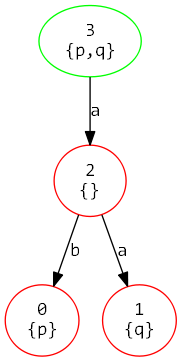
\includegraphics[scale=0.4]{example1.png}

\caption{The formula is satisfied in state $3$ (green) and unsatisfied in states $0, 1, 2$ (red). }
\end{figure}


\subsection{A PDL formula with Kripke frame}

\subsubsection*{Input}
\begin{verbatim}
K = {01,2,3,4,5}
m(p) = {01,2,4}
m(q) = {01, 3}
m(r) = {5}
m(a) = {(01,2), (01,4), (2,4), (01,3)}
m(b) = {(01,3), (3,3)}
m(c) = {(5,5)}
[a union b union c] (q and not p)
\end{verbatim}
The above formula is equivalent to:
\begin{align*}
[((a \cup b) \cup c)](q \wedge \neg p)
\end{align*}
\subsection*{Output (.kripke file)}
\begin{verbatim}
K = {s01, s2, s3, s4, s5}
m(p) = {s01, s2, s4}
m(q) = {s01, s3}
m(r) = {s5}
m(a) = {(s01,s2), (s01,s4), (s2,s4), (s01,s3)}
m(b) = {(s01,s3), (s3,s3)}
m(c) = {(s5,s5)}
Satisfying states: [s3, s4]
\end{verbatim}
\subsection*{Output (.dot file)}

\begin{figure}[H]
\center
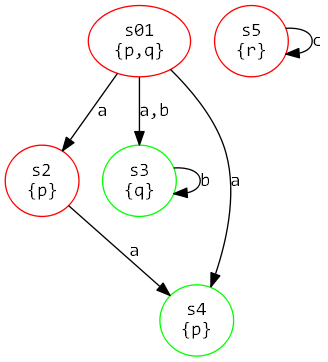
\includegraphics[scale=0.4]{example2.png}

\caption{The formula is satisfied in states $s3, s4$ (green) and unsatisfied in states $s01, s2, s5$ (red). }
\end{figure}


\subsection{A valid PDL formula}
\subsubsection*{Input}
\begin{verbatim}
not (<a converse> [a] p -> p)
\end{verbatim}
The above formula is equivalent to 
\begin{align*}
\neg(\langle a^{\_} \rangle [a] p \rightarrow p)
\end{align*}

\subsubsection*{Output}
unsat


This means the formula $\langle a^{\_} \rangle [a] p \rightarrow p$ is valid in all kripke frames.
\section{Benchmark}
To rigorously test the PDL solver, I used the valid formulas from chapter 5 as a benchmark. The total number of valid formulas in the benchmark is 42. The PDL solver managed to prove 24 formulas in less than 2 seconds, and timed out after 1 minute in 18 formulas.  I guess this benchmark can be used for the relation theory in CVC4. Table \ref{tab:benchmark} summarizes the result. 

\begin{table}[H]
\center
\begin{tabular}{lccr}
\toprule
Label & PDL formula & Output & Duration \\
\midrule
Book formula 1 & $\neg ([a](p \wedge q) \leftrightarrow  [a] p \wedge [a]q)$   & unknown   & 60,000 ms \\
Book formula 2 & $\neg ([a;b]p  \leftrightarrow  [a][b]p)$  & unknown   & 60,000 ms \\
Book formula 3 & $\neg ([\textit{if }p\textit{ then }a\textit{ else }b]p  \leftrightarrow  [\textit{if }\neg  p\textit{ then }b\textit{ else }a]p)$  & unknown   & 60,000 ms \\
	
Deductive system 2 & $\neg ([a](p \rightarrow  q) \rightarrow  ([a]p \rightarrow  [a]q))$  & unsat & 100 ms \\
	
Deductive system 3 & $\neg ([a](p \wedge q) \rightarrow  ([a]p \wedge [a]q))$  & unknown   & 60,000 ms \\
	
Deductive system 4 & $\neg ([a \cup b]p  \leftrightarrow  [a]p \wedge [b]p)$  & unknown   & 60,000 ms \\
	
Deductive system 5 & $\neg ([a;b]p  \leftrightarrow  [a][b]p)$  & unknown   & 60,000 ms \\
	
Deductive system 6 & $\neg ([q?]p  \leftrightarrow  (q \rightarrow  p))$  & unsat  & 77 ms \\
	
Deductive system 7 & $\neg (p \wedge [a][a^{*}] p  \leftrightarrow  [a^{*}]p)$  & unknown   & 60,000 ms \\
	
Deductive system 8 & $\neg (p \wedge [a^{*}](p \rightarrow  [a]p) \rightarrow  [a^{*}]p)$  & unknown   & 60,000 ms \\
	
Deductive system 9 MP & $\neg ((p \wedge (p \rightarrow  q)) \rightarrow  q)$  & unsat  & 73 ms \\
	

Theorem 6.1 & $\neg ( \langle  a \rangle  (p \vee q)  \leftrightarrow   \langle  a \rangle  p \vee  \langle  a \rangle  q)$  & unsat & 90 ms \\
	

Theorem 6.2 & $\neg ([a](p \wedge q)  \leftrightarrow  [a]p \wedge [a]q)$  & unknown   & 60,000 ms \\
	

Theorem 6.3 & $\neg ( \langle  a \rangle  p \wedge [a] q \rightarrow   \langle  a \rangle  (p \wedge q))$  & unsat & 78 ms \\
	

Theorem 6.4 & $\neg ([a](p \rightarrow  q) \rightarrow  ([a]p \rightarrow  [a] q))$  & unsat & 99 ms \\
	

Theorem 6.5 & $\neg ( \langle  a \rangle  (p \wedge q) \rightarrow   \langle  a \rangle   p \wedge  \langle  a \rangle   q)$  & unsat & 67 ms \\
	

Theorem 6.6 & $\neg ([a]p \vee [a] q \rightarrow  [a] (p \vee q))$  & unknown   & 60,000 ms \\
	

Theorem 6.7 & $\neg ( \langle  a \rangle   0  \leftrightarrow  0)$  & unsat & 57 ms \\
	

Theorem 6.8 & $\neg ([a]p  \leftrightarrow  \neg   \langle  a \rangle   \neg  p)$  & unsat & 95 ms \\
	

Theorem 8.1 & $\neg ( \langle  a \cup b \rangle   p  \leftrightarrow   \langle  a \rangle   p \vee  \langle  b \rangle   p)$  & unsat & 82 ms \\
	

Theorem 8.2 & $\neg ([a \cup b] p  \leftrightarrow  [a] p \wedge [b] p)$  & unknown   & 60,000 ms \\
	

Theorem 10.1 & $\neg ( \langle  a ; b \rangle   p  \leftrightarrow   \langle  a \rangle   \langle  b \rangle   p)$  & unsat  & 93 ms  \\
	

Theorem 10.2 & $\neg ([a ; b] p  \leftrightarrow  [a][b] p)$  & unknown   & 60,000 ms \\
	

Theorem 11.1 & $\neg ( \langle  p? \rangle   q  \leftrightarrow  p \wedge q)$  & unsat & 82 ms \\
	

Theorem 11.2 & $\neg ([p?] q  \leftrightarrow  (p \rightarrow  q))$  & unsat & 82 ms \\
	

Theorem 12.1 & $\neg ([p?] q  \leftrightarrow  (p \rightarrow  q))$  & unsat  & 80 ms \\
	

Theorem 15.1 & $\neg ([a^{*}]p \rightarrow  p)$  & unsat  & 66 ms \\
	

Theorem 15.2 & $\neg (p \rightarrow   \langle  a^{*} \rangle   p)$  & unsat & 68 ms \\
	

Theorem 15.3 & $\neg ([a^{*}]p \rightarrow  [a]p)$  & unsat & 74 ms \\
	

Theorem 15.4 & $\neg ( \langle  a \rangle  p \rightarrow   \langle  a^{*} \rangle  p)$  & unsat  & 71 ms \\
	

Theorem 15.5 & $\neg ([a^{*}]p  \leftrightarrow  [a^{*};a^{*}]p)$  & unsat &  1,200 ms\\
	

Theorem 15.6 & $\neg ( \langle  a^{*} \rangle  p  \leftrightarrow   \langle  a^{*};a^{*} \rangle  p)$  & unsat & 109ms \\
	

Theorem 15.7 & $\neg ([a^{*}]p  \leftrightarrow  [(a^*)^*]p)$  & unknown   & 60,000 ms \\
	

Theorem 15.8 & $\neg ( \langle  a^{*} \rangle  p  \leftrightarrow   \langle  (a^*)^* \rangle  p)$  & unknown   & 60,000 ms \\
	

Theorem 15.9 & $\neg ([a^{*}]p  \leftrightarrow  p \wedge [a][a^{*}]p)$  & unknown   & 60,000 ms \\
	

Theorem 15.10 & $\neg ( \langle  a^{*} \rangle  p  \leftrightarrow  p \vee  \langle  a \rangle   \langle  a^{*} \rangle  p)$  & unknown   & 60,000 ms \\
	

Theorem 15.11 & $\neg ([a^{*}]p  \leftrightarrow  p \wedge [a^{*}](p \rightarrow  [a]p))$  & unknown   & 60,000 ms \\
	

Theorem 15.12 & $\neg ( \langle  a^{*} \rangle  p  \leftrightarrow  p \vee  \langle  a^{*} \rangle  (\neg  p \wedge  \langle  a \rangle  p))$  & unknown   & 60,000 ms \\
theorem 13.1 & $\neg (p \rightarrow  [a] \langle  a^{\_} \rangle  p)$  & unsat & 375 ms \\
theorem 13.2 & $\neg (p \rightarrow  [a^{\_}] \langle  a \rangle  p)$  & unsat & 73 ms \\
theorem 13.3 & $\neg ( \langle  a \rangle  [a^{\_}]p \rightarrow  p)$  & unsat & 79 ms \\
theorem 13.4 & $\neg ( \langle  a^{\_} \rangle  [a]p \rightarrow  p)$  & unsat & 74 ms \\  
\bottomrule 
\end{tabular}
\caption{PDL solver results for 5 valid formulas in chapter 5 with  1 minute timeout.}
\label{tab:benchmark}
\end{table}

\bibliographystyle{plain}

\bibliography{references}

\end{document}
